\documentclass[16pt,b5paper]{article}

\title{TikZレシピ集}
\author{tomixy}

% === font ===

\usepackage[T1]{fontenc}

% normal font, math font
\usepackage[light,math]{anttor}

% monospace font
\usepackage[scaled]{beramono}

% === layout ===

\usepackage[margin=15mm]{geometry} % 余白
\renewcommand{\baselinestretch}{1.2} % 行間

% === code block ===

\usepackage{listings}
\usepackage{xcolor}

\definecolor{codegreen}{rgb}{0,0.6,0}
\definecolor{codegray}{rgb}{0.5,0.5,0.5}
\definecolor{codepurple}{rgb}{0.58,0,0.82}
\definecolor{backcolour}{rgb}{0.976,0.976,0.976}

\lstdefinestyle{mystyle}{
    backgroundcolor=\color{backcolour},   
    commentstyle=\color{codegreen},
    keywordstyle=\color{magenta},
    numberstyle=\tiny\color{codegray},
    stringstyle=\color{codepurple},
    basicstyle=\ttfamily\footnotesize,
    breakatwhitespace=false,         
    breaklines=true,                 
    captionpos=b,                    
    keepspaces=true,                 
    numbers=none,                    
    numbersep=5pt,                  
    showspaces=false, 
    showstringspaces=false,
    showtabs=false,                  
    tabsize=2,
    frame=shadowbox,
}

\lstset{style=mystyle}

% === tikz ===

\usepackage[dvipdfmx]{graphicx}
\usepackage{tikz} %図を描く
\usetikzlibrary{
  positioning,
  intersections,
  calc,
  arrows.meta,
  math,
  3d,
  bending,
  angles,
  quotes
}

\tikzstyle{axis}=[->, >=Stealth]
\tikzstyle{plotline}=[blue,very thick]
\tikzstyle{vector}=[->,>=Stealth,very thick, line cap=round]
\tikzstyle{zy-plane}=[canvas is zy plane at x=0]
\tikzstyle{xz-plane}=[canvas is xz plane at y=0]
\tikzstyle{xy-plane}=[canvas is xy plane at z=0]

\usepackage[outline]{contour} % 文字の縁取り

% ---

\begin{document}

\maketitle
\tableofcontents

\section{TikZで線を描く}

\subsection{線分}

\begin{tikzpicture}[scale=1]
  \draw (0,0)--(3,2);
\end{tikzpicture}

\begin{lstlisting}
  \begin{tikzpicture}[scale=1]
    \draw (0,0)--(3,2);
  \end{tikzpicture}
\end{lstlisting}

\begin{itemize}
  \item 複数の点を結ぶには\verb|--|を使う
\end{itemize}

\subsection{中央寄せ}

\begin{center}
  \begin{tikzpicture}[scale=1]
    \draw (0,0)--(3,2);
  \end{tikzpicture}
\end{center}

\begin{lstlisting}
  \begin{center}
    \begin{tikzpicture}[scale=1]
      \draw (0,0)--(3,2);
    \end{tikzpicture}
  \end{center}
\end{lstlisting}

\begin{itemize}
  \item \verb|\begin{center}...\end{center}|で中央寄せ
\end{itemize}

\subsection{折れ線}

\begin{tikzpicture}[scale=0.75]
  \draw (0,0)--(3,2)--(5,-2);
\end{tikzpicture}

\begin{lstlisting}
  \draw (0,0)--(3,2)--(5,-2);
\end{lstlisting}

\subsection{点線や二重線}

\begin{tikzpicture}[scale=0.75]
  \draw[very thick,dotted] (0,0)--(3,2)--(5,-2);
  \draw[very thick,dashed] (0+6,0)--(3+6,2)--(5+6,-2);
  \draw[very thick,double] (0+12,0)--(3+12,2)--(5+12,-2);
\end{tikzpicture}

\begin{lstlisting}
  \draw[very thick,dotted] (0,0)--(3,2)--(5,-2);
  \draw[very thick,dashed] (0+6,0)--(3+6,2)--(5+6,-2);
  \draw[very thick,double] (0+12,0)--(3+12,2)--(5+12,-2);
\end{lstlisting}

\begin{itemize}
  \item 3 + 6のような計算式で座標を指定することも可能
\end{itemize}

\subsection{矢印}

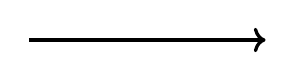
\begin{tikzpicture}[scale=1]
  \draw[->,very thick](0,0)--(3,0);
\end{tikzpicture}

\begin{lstlisting}
  \draw[->,very thick](0,0)--(3,0);
\end{lstlisting}

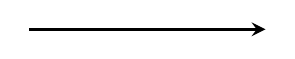
\begin{tikzpicture}[scale=1]
  \draw[->,>=stealth,very thick](0,0)--(3,0);
\end{tikzpicture}

\begin{lstlisting}
  \draw[->,>=stealth,very thick](0,0)--(3,0);
\end{lstlisting}

\subsection{三角形}

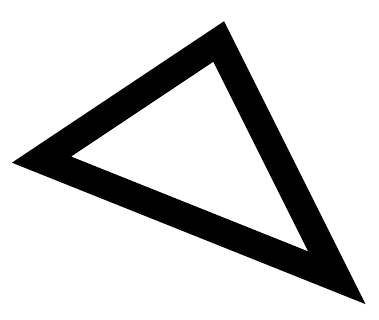
\begin{tikzpicture}[scale=0.75]
  \draw[line width=10pt] (0,0)--(3,2)--(5,-2)--cycle;
\end{tikzpicture}

\begin{lstlisting}
  \draw[line width=10pt] (0,0)--(3,2)--(5,-2)--cycle;
\end{lstlisting}

\begin{itemize}
  \item \verb|cycle|を指定することで、最後の点と最初の点を結ぶ
\end{itemize}

\subsection{弧}

\begin{tikzpicture}[scale=2]
  \draw[dashed] (0,0) to [out=30,in=150] (3,0);
\end{tikzpicture}

\begin{lstlisting}
  \draw[dashed] (0,0) to [out=30,in=150] (3,0);
\end{lstlisting}

\begin{itemize}
  \item 始点での角度と終点での角度を指定している
  \item \verb|[out=30,in=150]|は、「始点では30°の方向に出て、終点では150°の方向から入る」
\end{itemize}

\subsection{図の中に文字}

\begin{tikzpicture}[scale=0.75]
  \draw (0,0)--(3,2)--(5,-2)--cycle;
  \draw (0,0) node[left]{A};
  \draw (3,2) node[above]{B};
  \draw (5,-2) node[below right]{C};
\end{tikzpicture}

\begin{lstlisting}
  \draw (0,0)--(3,2)--(5,-2)--cycle;
  \draw (0,0) node[left]{A};
  \draw (3,2) node[above]{B};
  \draw (5,-2) node[below right]{C};
\end{lstlisting}

\begin{itemize}
  \item 図に文字を入れるときは\verb|node|コマンドを使う
\end{itemize}

\subsection{図の中に数式}

\begin{tikzpicture}[scale=0.75]
  \draw (0,0)--(3,2)--(5,-2)--cycle;
  \draw (0,0) node[left]{A};
  \draw (3,2) node[above]{B$(\beta=3+2i)$};
  \draw (5,-2) node[below right]{C};
\end{tikzpicture}

\begin{lstlisting}
  \draw (0,0)--(3,2)--(5,-2)--cycle;
  \draw (0,0) node[left]{A};
  \draw (3,2) node[above]{B$(\beta=3+2i)$};
  \draw (5,-2) node[below right]{C};
\end{lstlisting}

\subsection{図形と重なる文字}

\begin{tikzpicture}[scale=2]
  \draw (0,0)--(3,0);
  \draw[dashed] (0,0) to [out=30,in=150] (3,0);
  \draw (1.5,0.45) node {3};
\end{tikzpicture}

\begin{lstlisting}
  \draw (0,0)--(3,0);
  \draw[dashed] (0,0) to [out=30,in=150] (3,0);
  \draw (1.5,0.45) node {3};
\end{lstlisting}

\begin{itemize}
  \item 「3」の背景を白で塗りつぶしたい
  \item そのためには、\verb|node|に\verb|[fill=white]|を追加する
\end{itemize}

\begin{tikzpicture}[scale=2]
  \draw (0,0)--(3,0);
  \draw[dashed] (0,0) to [out=30,in=150] (3,0);
  \draw (1.5,0.45) node[fill=white]{3};
\end{tikzpicture}

\begin{lstlisting}
  \draw (0,0)--(3,0);
  \draw[dashed] (0,0) to [out=30,in=150] (3,0);
  \draw (1.5,0.45) node[fill=white]{3};
\end{lstlisting}

\section{TikZでグラフを描く}

\subsection{座標軸}

\begin{tikzpicture}[scale=1]
  \draw[->,>=stealth,semithick] (-3,0)--(3,0) node[right]{$x$}; %x軸
  \draw[->,>=stealth,semithick] (0,-1)--(0,4) node[left]{$y$}; %y軸
  \draw (0,0) node[below left]{O}; %原点
\end{tikzpicture}

\begin{lstlisting}
  \draw[->,>=stealth,semithick] (-3,0)--(3,0) node[right]{$x$}; %x軸
  \draw[->,>=stealth,semithick] (0,-1)--(0,4) node[left]{$y$}; %y軸
  \draw (0,0) node[below left]{O}; %原点
\end{lstlisting}

\subsection{関数のグラフ}

\begin{tikzpicture}[scale=1]
  % 座標軸
  \draw[->,>=stealth,semithick] (-3,0)--(3,0) node[right]{$x$}; %x軸
  \draw[->,>=stealth,semithick] (0,-1)--(0,4) node[left]{$y$}; %y軸
  \draw (0,0) node[below left]{O}; %原点
  % グラフ
  \draw plot(\x,\x/2+1);
\end{tikzpicture}

\begin{lstlisting}
  \draw plot(\x,\x/2+1);
\end{lstlisting}

\subsection{定義域の指定}

\begin{tikzpicture}[scale=1]
  % 座標軸
  \draw[->,>=stealth,semithick] (-3,0)--(3,0) node[right]{$x$}; %x軸
  \draw[->,>=stealth,semithick] (0,-1)--(0,4) node[left]{$y$}; %y軸
  \draw (0,0) node[below left]{O}; %原点
  % グラフ
  \draw[thick,domain=-3:3] plot(\x,\x/2+1);
\end{tikzpicture}

\begin{lstlisting}
  \draw[thick,domain=-3:3] plot(\x,\x/2+1);
\end{lstlisting}

\subsection{滑らかな曲線}

\begin{tikzpicture}[scale=1,samples=300]
  % 座標軸
  \draw[->,>=stealth,semithick] (-4,0)--(4,0) node[right]{$x$}; %x軸
  \draw[->,>=stealth,semithick] (0,-3)--(0,3) node[left]{$y$}; %y軸
  \draw (0,0) node[below left]{O}; %原点
  % グラフ
  \draw[thick,domain=-4:4] plot(\x,{2*sin(\x r)});
\end{tikzpicture}

\begin{lstlisting}
  \begin{tikzpicture}[scale=1,samples=300]
    \draw[thick,domain=-4:4] plot(\x,{2*sin(\x r)});
  \end{tikzpicture}
\end{lstlisting}

\begin{itemize}
  \item \verb|samples|でplotする点を増やすと、カクカクを回避できる
\end{itemize}

\subsection{指定した範囲内のみ描画}

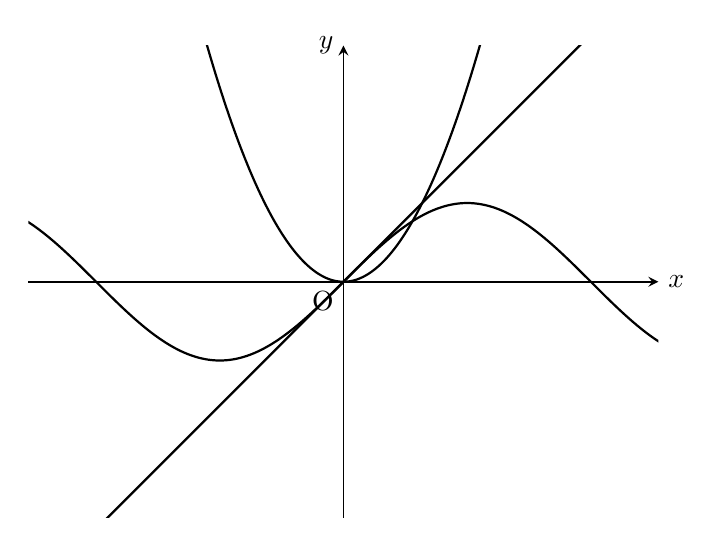
\begin{tikzpicture}[scale=1,samples=300]
  % 座標軸
  \draw[->,>=stealth,semithick] (-4,0)--(4,0) node[right]{$x$}; %x軸
  \draw[->,>=stealth,semithick] (0,-3)--(0,3) node[left]{$y$}; %y軸
  \draw (0,0) node[below left]{O}; %原点
  % グラフ
  \begin{scope} \clip (-4,-3) rectangle (4,3);
    \draw[thick] plot(\x,{sin(\x r)});
    \draw[thick] plot(\x,{pow(\x,2)});
    \draw[thick] plot(\x,\x);
  \end{scope}
\end{tikzpicture}

\begin{lstlisting}
  \begin{scope} \clip (-4,-3) rectangle (4,3);
    \draw[thick] plot(\x,{sin(\x r)});
    \draw[thick] plot(\x,{pow(\x,2)});
    \draw[thick] plot(\x,\x);
  \end{scope}
\end{lstlisting}

\begin{itemize}
  \item 複数の関数それぞれに定義域を指定するのは面倒
  \item \verb|scope|環境の\verb|\clip|コマンドで、指定した長方形の範囲内のみ描画できる
\end{itemize}

\subsection{グラフに関数名を表示}

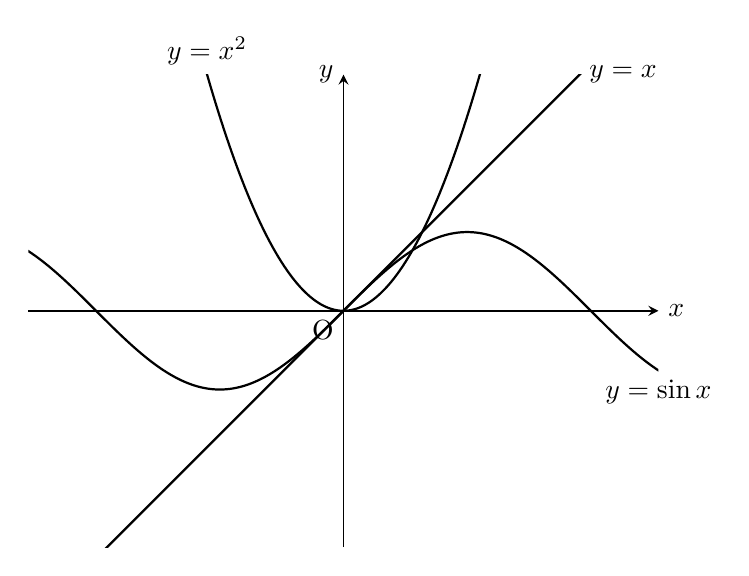
\begin{tikzpicture}[scale=1,samples=300]
  % 座標軸
  \draw[->,>=stealth,semithick] (-4,0)--(4,0) node[right]{$x$}; %x軸
  \draw[->,>=stealth,semithick] (0,-3)--(0,3) node[left]{$y$}; %y軸
  \draw (0,0) node[below left]{O}; %原点
  % グラフ
  \begin{scope} \clip (-4,-3) rectangle (4,3);
    \draw[thick] plot(\x,{sin(\x r)});
    \draw[thick] plot(\x,{pow(\x,2)});
    \draw[thick] plot(\x,\x);
  \end{scope}
  % 関数名
  \draw ({-sqrt(3)},3) node[above]{$y=x^2$};
  \draw (3,3) node[right]{$y=x$};
  \draw (4,{sin(4 r)}) node[below]{$y=\sin x$};
\end{tikzpicture}

\begin{lstlisting}
  % グラフ
  \begin{scope} \clip (-4,-3) rectangle (4,3);
    \draw[thick] plot(\x,{sin(\x r)});
    \draw[thick] plot(\x,{pow(\x,2)});
    \draw[thick] plot(\x,\x);
  \end{scope}
  
  % 関数名
  \draw ({-sqrt(3)},3) node[above]{$y=x^2$};
  \draw (3,3) node[right]{$y=x$};
  \draw (4,{sin(4 r)}) node[below]{$y=\sin x$};
\end{lstlisting}

\begin{itemize}
  \item 座標軸や各グラフの式などは\verb|scope|環境の外に書かないと、切り取られてしまうことがあるので注意
\end{itemize}

\section{TikZでの頂点定義}

\subsection{1点からのびる複数の線}

\begin{tikzpicture}[scale=1]
  \coordinate[label=left:A] (A) at (-1,2);
  \draw (A) -- (3,3) node[right]{B};
  \draw (A) -- (4,1) node[right]{C};
  \draw (A) -- (3,0) node[right]{D};
  \draw (A) -- (1,-2) node[right]{E};
\end{tikzpicture}

\begin{lstlisting}
  \coordinate[label=left:A] (A) at (-1,2);
  \draw (A) -- (3,3) node[right]{B};
  \draw (A) -- (4,1) node[right]{C};
  \draw (A) -- (3,0) node[right]{D};
  \draw (A) -- (1,-2) node[right]{E};
\end{lstlisting}

\begin{itemize}
  \item \verb|\coordinate|で点(-1,2)にAという名前をつけている
  \item 点Aに名前をつけることで、点Aの位置を変えたいときに書き換え箇所が1箇所で済む
\end{itemize}

\subsection{正多角形}

\begin{tikzpicture}[scale=2]
  \coordinate (A) at (0,1);
  \coordinate (B) at ({cos(9*pi/10 r)},{sin(9*pi/10 r)});
  \coordinate (C) at ({cos(13*pi/10 r)},{sin(13*pi/10 r)});
  \coordinate (D) at ({cos(17*pi/10 r)},{sin(17*pi/10 r)});
  \coordinate (E) at ({cos(21*pi/10 r)},{sin(21*pi/10 r)});

  \draw (A)--(B)--(C)--(D)--(E)--cycle;
\end{tikzpicture}

\begin{lstlisting}
  % 頂点の定義
  \coordinate (A) at (0,1);
  \coordinate (B) at ({cos(9*pi/10 r)},{sin(9*pi/10 r)});
  \coordinate (C) at ({cos(13*pi/10 r)},{sin(13*pi/10 r)});
  \coordinate (D) at ({cos(17*pi/10 r)},{sin(17*pi/10 r)});
  \coordinate (E) at ({cos(21*pi/10 r)},{sin(21*pi/10 r)});

  % 頂点を結ぶ
  \draw (A)--(B)--(C)--(D)--(E)--cycle;
\end{lstlisting}

\begin{itemize}
  \item \verb|\coordinate|で頂点を定義してから、\verb|\draw|で結ぶ
\end{itemize}

\subsection{対角線を引いた正多角形}

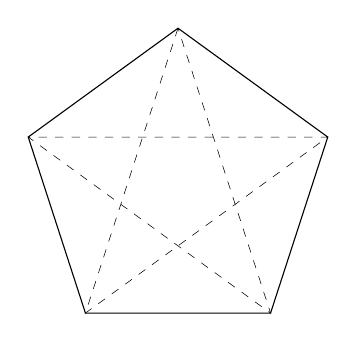
\begin{tikzpicture}[scale=2]
  % 頂点の定義
  \coordinate (A) at (0,1);
  \coordinate (B) at ({cos(9*pi/10 r)},{sin(9*pi/10 r)});
  \coordinate (C) at ({cos(13*pi/10 r)},{sin(13*pi/10 r)});
  \coordinate (D) at ({cos(17*pi/10 r)},{sin(17*pi/10 r)});
  \coordinate (E) at ({cos(21*pi/10 r)},{sin(21*pi/10 r)});

  % 頂点を結ぶ
  \draw (A)--(B)--(C)--(D)--(E)--cycle;
  % 対角線を引く
  \draw[very thin,dashed] (A)--(C)--(E)--(B)--(D)--cycle;
\end{tikzpicture}

\begin{lstlisting}
  % 頂点の定義
  \coordinate (A) at (0,1);
  \coordinate (B) at ({cos(9*pi/10 r)},{sin(9*pi/10 r)});
  \coordinate (C) at ({cos(13*pi/10 r)},{sin(13*pi/10 r)});
  \coordinate (D) at ({cos(17*pi/10 r)},{sin(17*pi/10 r)});
  \coordinate (E) at ({cos(21*pi/10 r)},{sin(21*pi/10 r)});

  % 頂点を結ぶ
  \draw (A)--(B)--(C)--(D)--(E)--cycle;
  % 対角線を引く
  \draw[very thin,dashed] (A)--(C)--(E)--(B)--(D)--cycle;
\end{lstlisting}

\begin{itemize}
  \item \verb|\coordinate|で点を定義しておけば、\verb|\draw|を増やすだけでいろいろな線を引ける
\end{itemize}

\section{TikZでの繰り返し}

\subsection{頂点をコードで生成する}

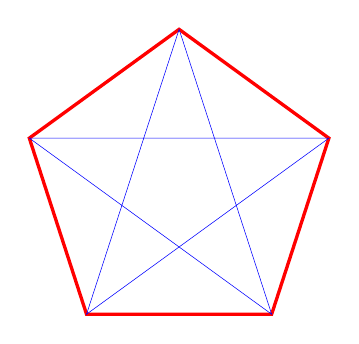
\begin{tikzpicture}[scale=2]
  % kは1から5まで動く
  % A_1からA_5までの座標が生成される
  \foreach \k in{1,...,5}
  \coordinate (A_\k) at ({cos((4*\k+1)*pi/10 r)},{sin((4*\k+1)*pi/10 r)});

  % 頂点を結んで描画
  \draw[red,very thick] (A_1)--(A_2)--(A_3)--(A_4)--(A_5)--cycle;
  \draw[blue,very thin] (A_1)--(A_3)--(A_5)--(A_2)--(A_4)--cycle;
\end{tikzpicture}

\begin{lstlisting}
  % 頂点の生成
  \foreach \k in{1,...,5}
  \coordinate (A_\k) at ({cos((4*\k+1)*pi/10 r)},{sin((4*\k+1)*pi/10 r)});

  % 頂点を結んで図形を描画
  \draw[red,very thick] (A_1)--(A_2)--(A_3)--(A_4)--(A_5)--cycle;
  \draw[blue,very thin] (A_1)--(A_3)--(A_5)--(A_2)--(A_4)--cycle;
\end{lstlisting}

\begin{itemize}
  \item \verb|\foreach|文で頂点を動的に生成する
  \item \verb|\k|は1から5まで動き、\verb|A_1|から\verb|A_5|までの座標が生成される
\end{itemize}

\subsection{各点に連番を振る}

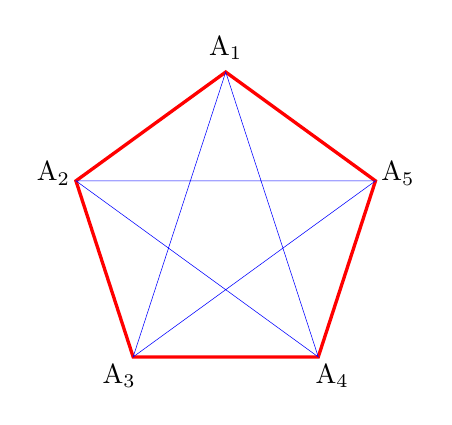
\begin{tikzpicture}[scale=2]
  \foreach \k in{1,...,5}
  \coordinate (A_\k) at ({cos((4*\k+1)*pi/10 r)},{sin((4*\k+1)*pi/10 r)});

  \foreach \k in{1,...,5} \draw ($(0,0)!1.15!(A_\k)$) node{$\mathrm{A_\k}$};

  \draw[red,very thick] (A_1)--(A_2)--(A_3)--(A_4)--(A_5)--cycle;
  \draw[blue,very thin] (A_1)--(A_3)--(A_5)--(A_2)--(A_4)--cycle;
\end{tikzpicture}

\begin{lstlisting}
  % 頂点の生成
  \foreach \k in{1,...,5}
  \coordinate (A_\k) at ({cos((4*\k+1)*pi/10 r)},{sin((4*\k+1)*pi/10 r)});

  % ラベルの描画
  \foreach \k in{1,...,5} \draw ($(0,0)!1.15!(A_\k)$) node{$\mathrm{A_\k}$};

  % 図形の描画
  \draw[red,very thick] (A_1)--(A_2)--(A_3)--(A_4)--(A_5)--cycle;
  \draw[blue,very thin] (A_1)--(A_3)--(A_5)--(A_2)--(A_4)--cycle;
\end{lstlisting}

\begin{itemize}
  \item \verb|$(0,0)!1.15!(A_\k)$|は、点\verb|(0,0)|から点\verb|(A_k)|の方向に1.15進んだ点を表す
\end{itemize}

\section{TikZで円を描く}

\subsection{円}

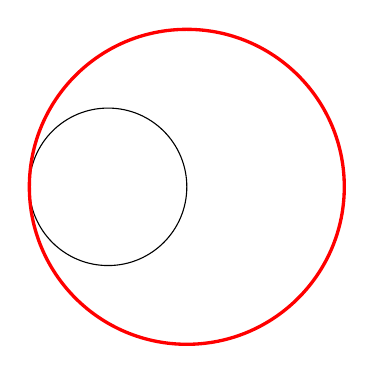
\begin{tikzpicture}
  \draw (0,0) circle[radius=1];
  \draw [red,very thick](1,0)circle[radius=2];
\end{tikzpicture}

\begin{lstlisting}
  \draw (0,0) circle[radius=1];
  \draw [red,very thick](1,0)circle[radius=2];
\end{lstlisting}

\begin{itemize}
  \item \verb|\draw 中心 circle[radius=半径]|
  \item TikZでは原則「入力した順」に描かれているため、後から入力したものが上に重なる
\end{itemize}

\subsection{楕円}

\begin{tikzpicture}
  \draw(0,0) circle (3 and 2);
\end{tikzpicture}

\begin{lstlisting}
  \draw(0,0) circle (3 and 2);
\end{lstlisting}

\begin{itemize}
  \item \verb|\draw 中心 circle (x半径 and y半径)]|
\end{itemize}

\section{TikZで図形を塗りつぶす}

\subsection{縁取りなしで塗りつぶされた円}


\begin{tikzpicture}
  \fill [cyan] (0,0) circle [radius=2];
\end{tikzpicture}

\begin{lstlisting}
  \fill [cyan] (0,0) circle [radius=2];
\end{lstlisting}

\begin{itemize}
  \item \verb|\fill|は縁取りなしで塗りつぶす
\end{itemize}

\subsection{縁取り付きで塗りつぶされた円}

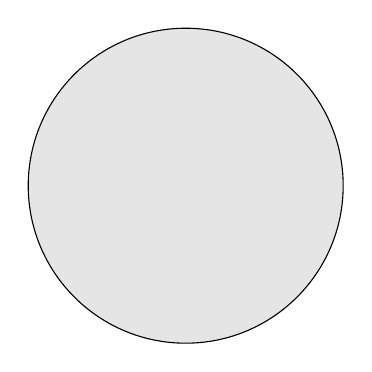
\begin{tikzpicture}
  \filldraw [fill=black!10!white] (0,0) circle [radius=2];
\end{tikzpicture}

\begin{lstlisting}
  \filldraw [fill=black!10!white] (0,0) circle [radius=2];
\end{lstlisting}

\begin{itemize}
  \item \verb|\filldraw|は縁取り付きで塗りつぶす
  \item \verb|black!10!white|は「黒を白に10\%混ぜた色」
\end{itemize}

\section{TikZでグリッド線を描く}

\subsection{xy座標平面}

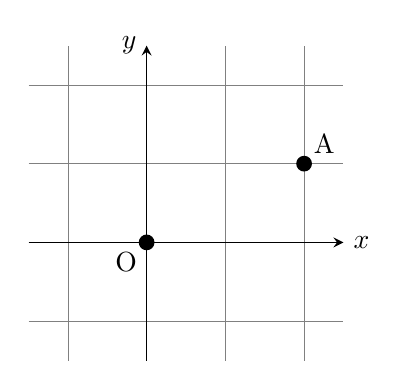
\begin{tikzpicture}
  % グリッド線
  \draw [step=1,very thin,gray] (-1.5,-1.5) grid (2.5,2.5);

  % 座標軸
  \draw [->,>=stealth,semithick] (-1.5,0)--(2.5,0) node[right]{$x$};
  \draw [->,>=stealth,semithick] (0,-1.5)--(0,2.5) node[left]{$y$};

  % 原点
  \draw (0,0) node[below left]{O};

  % 座標平面上の点
  \fill (0,0) circle [radius=0.1];
  \fill (2,1) circle [radius=0.1] node[above right]{A};
\end{tikzpicture}

\begin{lstlisting}
  % グリッド線
  \draw [step=1,very thin,gray] (-1.5,-1.5) grid (2.5,2.5);

  % 座標軸
  \draw [->,>=stealth,semithick] (-1.5,0)--(2.5,0) node[right]{$x$};
  \draw [->,>=stealth,semithick] (0,-1.5)--(0,2.5) node[left]{$y$};

  % 原点
  \draw (0,0) node[below left]{O};

  % 座標平面上の点
  \fill (0,0) circle [radius=0.1];
  \fill (2,1) circle [radius=0.1] node[above right]{A};
\end{lstlisting}

\section{TikZでベン図を描く}

\subsection{塗りつぶしなしのベン図}

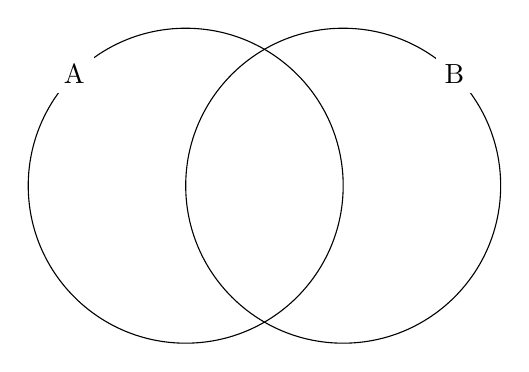
\begin{tikzpicture}[scale=2]
  % ベン図の円(集合)
  \draw (0,0) circle [radius=1];
  \draw (1,0) circle [radius=1];
  % 各集合のラベル
  \draw ({cos(pi*3/4 r)},{sin(pi*3/4 r)}) node[fill=white]{A};
  \draw ({1+cos(pi/4 r)},{sin(pi/4 r)}) node[fill=white]{B};
\end{tikzpicture}

\begin{lstlisting}
  % 集合を表すベン図の円(円周のみ)
  \draw (0,0) circle [radius=1];
  \draw (1,0) circle [radius=1];
  
  % 各集合のラベル
  \draw ({cos(pi*3/4 r)},{sin(pi*3/4 r)}) node[fill=white]{A};
  \draw ({1+cos(pi/4 r)},{sin(pi/4 r)}) node[fill=white]{B};
\end{lstlisting}

\subsection{共通部分だけ塗りつぶす}

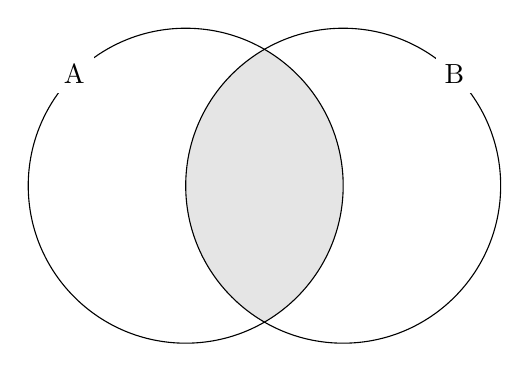
\begin{tikzpicture}[scale=2]
  % 片方の円で切り取り
  \begin{scope} \clip (1,0) circle [radius=1];
    % 両方の円を塗りつぶし
    \fill[black!10!] (0,0) circle [radius=1];
    \fill[black!10!] (0,0) circle [radius=1];
  \end{scope}

  % 集合を表すベン図の円(円周のみ)
  \draw (0,0) circle [radius=1];
  \draw (1,0) circle [radius=1];

  % 各集合のラベル
  \draw ({cos(pi*3/4 r)},{sin(pi*3/4 r)}) node[fill=white]{A};
  \draw ({1+cos(pi/4 r)},{sin(pi/4 r)}) node[fill=white]{B};
\end{tikzpicture}

\begin{lstlisting}
  % 片方の円で切り取り
  \begin{scope} \clip (1,0) circle [radius=1];
    % 両方の円を塗りつぶし
    \fill[black!10!] (0,0) circle [radius=1];
    \fill[black!10!] (0,0) circle [radius=1];
  \end{scope}

  % 集合を表すベン図の円(円周のみ)
  \draw (0,0) circle [radius=1];
  \draw (1,0) circle [radius=1];

  % 各集合のラベル
  \draw ({cos(pi*3/4 r)},{sin(pi*3/4 r)}) node[fill=white]{A};
  \draw ({1+cos(pi/4 r)},{sin(pi/4 r)}) node[fill=white]{B};
\end{lstlisting}

\begin{itemize}
  \item TikZでは原則「入力した順」に描かれるため、円周を描く前に内部を塗りつぶす
\end{itemize}

\section{TikZによる領域の図示}

\subsection{線分で囲まれた領域の図示}

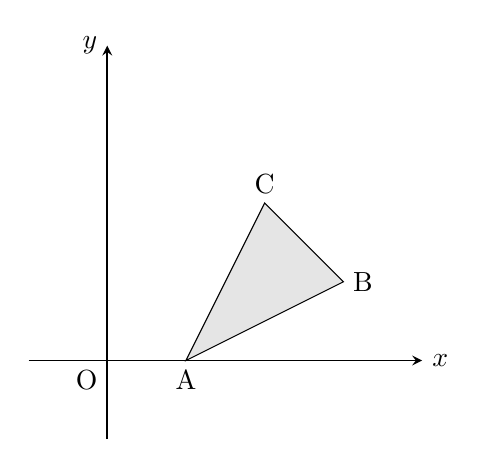
\begin{tikzpicture}[scale=1]
  % 三角形の頂点
  \coordinate[label=below:A] (A) at (1,0);
  \coordinate[label=right:B] (B) at (3,1);
  \coordinate[label=above:C] (C) at (2,2);

  % 三角形の描画(塗りつぶし)
  \filldraw[fill=gray!20!white] (A)--(B)--(C)--cycle;

  % 座標軸
  \draw[->,>=stealth,semithick] (-1,0)--(4,0) node[right]{$x$};
  \draw[->,>=stealth,semithick] (0,-1)--(0,4) node[left]{$y$};

  % 原点
  \draw(0,0) node[below left]{O};
\end{tikzpicture}

\begin{lstlisting}
  % 三角形の頂点
  \coordinate[label=below:A] (A) at (1,0);
  \coordinate[label=right:B] (B) at (3,1);
  \coordinate[label=above:C] (C) at (2,2);

  % 三角形の描画(塗りつぶし)
  \filldraw[fill=gray!20!white] (A)--(B)--(C)--cycle;

  % 座標軸
  \draw[->,>=stealth,semithick] (-1,0)--(4,0) node[right]{$x$};
  \draw[->,>=stealth,semithick] (0,-1)--(0,4) node[left]{$y$};

  % 原点
  \draw(0,0) node[below left]{O};
\end{lstlisting}

\begin{itemize}
  \item 線分に囲まれた多角形を塗りつぶすだけ
\end{itemize}

\subsection{関数グラフの囲む領域の図示}

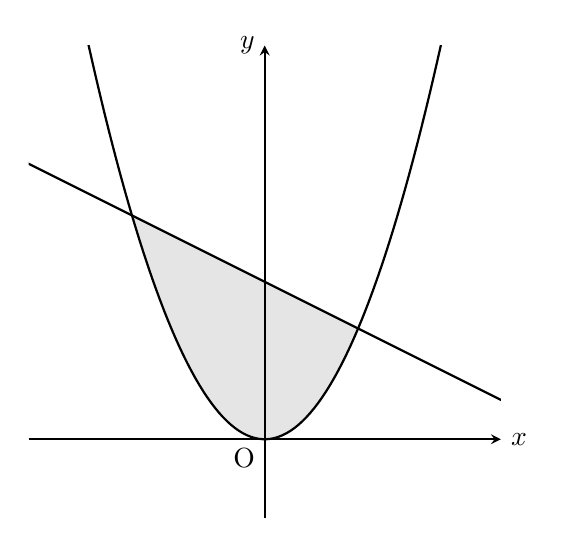
\begin{tikzpicture}[samples=200,scale=1]
  \begin{scope}\clip (-3,-1) rectangle (3,5);
    % 放射線
    \path[name path=C] plot(\x,{pow(\x,2)});
    % 直線
    \path[name path=L] plot(\x,-\x/2+2);
    % 放物線と直線の交点
    \path[name intersections={of= C and L,by={A,B}}];
    % pt単位の各点を座標に変換
    \tikzmath{
      coordinate \c; \c{A} = (A); \c{B} = (B); \c{U} = (1,1);
      \xA = \cx{A}/\cx{U}; \xB = \cx{B}/\cx{U};
    }
    % 関数の描画と塗りつぶし
    \fill[gray!20!white] plot[domain=\xA:\xB](\x,{pow(\x,2)});
    \draw[thick] plot(\x,{pow(\x,2)});
    \draw[thick] plot(\x,-\x/2+2);
  \end{scope}

  % 座標軸
  \draw[->,>=stealth,semithick] (-3,0)--(3,0)node[right]{$x$};
  \draw[->,>=stealth,semithick] (0,-1)--(0,5)node[left]{$y$};
  % 原点
  \draw (0,0)node[below left]{O};
\end{tikzpicture}

\begin{lstlisting}
  \begin{scope}\clip (-3,-1) rectangle (3,5);
    % 放射線
    \path[name path=C] plot(\x,{pow(\x,2)});
    % 直線
    \path[name path=L] plot(\x,-\x/2+2);
    % 放物線と直線の交点
    \path[name intersections={of= C and L,by={A,B}}];
    % pt単位の各点を座標に変換
    \tikzmath{
      coordinate \c; \c{A} = (A); \c{B} = (B); \c{U} = (1,1);
      \xA = \cx{A}/\cx{U}; \xB = \cx{B}/\cx{U};
    }
    % 関数の描画と塗りつぶし
    \fill[gray!20!white] plot[domain=\xA:\xB](\x,{pow(\x,2)});
    \draw[thick] plot(\x,{pow(\x,2)});
    \draw[thick] plot(\x,-\x/2+2);
  \end{scope}

  % 座標軸
  \draw[->,>=stealth,semithick] (-3,0)--(3,0)node[right]{$x$};
  \draw[->,>=stealth,semithick] (0,-1)--(0,5)node[left]{$y$};
  % 原点
  \draw (0,0)node[below left]{O};
\end{lstlisting}

\section{3Dの実例}

\def\xang{-13}
\def\zang{45}
\begin{tikzpicture}[x=(\xang:0.9), y=(90:0.9), z=(\zang:1.1)]
  \def\xmax{8.8}         % max x axis
  \def\ymin{-1.5}        % min y axis
  \def\ymax{1.6}         % max y axis
  \def\zmax{1.6}         % max z axis
  \def\xf{1.17*\xmax}    % x position frequency axis
  \def\A{(0.70*\ymax)}   % amplitude
  \def\T{(0.335*\xmax)}  % period
  \def\w{\zmax/11.2}     % spacing components
  \def\ang{47}           % angle
  \def\s{\ang/360*\T}    % time component
  \def\x{\A*cos(\ang)}   % real component
  \def\y{\A*sin(\ang)}   % imaginary component
  \def\N{100}            % number of samples
  \def\tick#1#2{\draw[thick] (#1) ++ (#2:0.12) --++ (#2-180:0.24)}

  % COMPLEX PLANE
  \begin{scope}[shift={(-1.6*\zmax,0,0)}]
    % 複素平面の枠
    \draw[black,fill=white,opacity=0.3,zy-plane](-1.25*\zmax,-1.25*\ymax) rectangle (1.4*\zmax,1.25*\ymax);
    % Im axis
    \draw[axis] (0,\ymin,0) -- (0,\ymax+0.02,0) node[pos=1,left=0,zy-plane] {Im};
    % Re axis
    \draw[axis] (0,0,-\zmax) -- (0,0,\zmax+0.02) node[right=1,below=0,zy-plane] {Re} coordinate (X);
    % 複素平面上の単位円
    \draw[plotline,zy-plane] (0,0) circle(0.991*\A) coordinate (O);
    % 単位円上の点P
    \fill[red,zy-plane] (\ang:{\A}) circle(0.07) coordinate(P);
    \node[blue,zy-plane,anchor=south west,scale=0.7] at (P) {$z(t)=Ae^{i\omega t}$};
    % 動径OP
    \draw[vector,thick,zy-plane] (0,0) -- (\ang:{\A-0.03}) coordinate (R);
    % 偏角を表す円弧
    \draw pic[-{>[flex'=1]},draw=blue,angle radius=14,angle eccentricity=1,"$\omega t$"{above=0,right=-0.5,yslant=0.69,scale=0.8},blue,zy-plane] {angle = X--O--R};
    % Re軸上の目盛り
    \tick{0,0,{\A}}{90};
    \tick{0,0,{-\A}}{90};
    % Im軸上の目盛り
    \tick{0,{\A},0}{\zang};
    \tick{0,{-\A},0}{\zang};
  \end{scope}

  % IMAGINARY
  \begin{scope}[shift={(0,0,1.9*\zmax)}]
    % sinを描く平面の枠
    \draw[black,fill=white,opacity=0.3,xy-plane](-0.5*\ymax,-1.2*\ymax) rectangle (1.10*\xmax,1.25*\ymax);
    % t axis
    \draw[axis] (-0.3*\ymax,0,0) -- (\xmax,0,0) node[below right,xy-plane] {$t$ [s]};
    % Im axis
    \draw[axis] (0,\ymin,0) -- (0,\ymax,0) node[left,xy-plane] {Im};
    % sin関数のグラフ
    \draw[plotline,samples=\N,smooth,variable=\t,domain=-0.05*\T:0.95*\xmax] plot(\t,{\A*sin(360/\T*\t)},0);
    % sin関数上の点I
    \fill[red,xy-plane] ({\s},{\y}) circle(0.07) coordinate(I);
    % 点Iでの波の高さを示すベクトル
    \draw[vector,thick,xy-plane] ({\s},0) --++ (0,{\y-0.03});
    \node[xy-plane,below] at ({\s},0) {$\omega t$};
    % 波の高さを表すIm軸上の目盛り
    \tick{0,{\A},0}{180};
    \tick{0,{-\A},0}{180};
    % 周期を示す目盛り
    \tick{{\T},0,0}{90} node[right=0,below,xy-plane] {\contour{white}{$T$}};
    \tick{{2*\T},0,0}{90} node[right=0,below,xy-plane] {\contour{white}{$2T$}};
    % 関数を表す数式
    \node[blue,below=0,xy-plane] at (0.4*\xmax,1.15*\ymax,0) {$y(t)=A\sin(\omega t)$};
  \end{scope}

  % REAL
  \begin{scope}[shift={(0,-1.8*\zmax,0)}]
    % cosを描く平面の枠
    \draw[black,fill=white,opacity=0.3,xz-plane] (-0.5*\ymax,-1.4*\ymax) rectangle (1.10*\xmax,1.25*\ymax);
    % t axis
    \draw[axis] (-0.3*\ymax,0,0) -- (\xmax,0,0) node[below right,xz-plane] {$t$ [s]};
    % Re axis
    \draw[axis] (0,0,-\zmax) -- (0,0,\zmax) node[left=-1,xz-plane] {Re};
    % cos関数のグラフ
    \draw[plotline,samples=\N,smooth,variable=\t,domain=-0.05*\T:0.95*\xmax] plot(\t,0,{\A*cos(360/\T*\t)});
    % cos関数上の点R
    \fill[red,xz-plane] ({\s},{\x}) circle(0.07) coordinate(R);
    % 点Rでの波の高さを示すベクトル
    \draw[vector,thick,xz-plane] ({\s},0) --++ (0,{\x-0.03});
    \node[xz-plane,below] at ({\s},0) {$\omega t$};
    % 波の高さを表すRe軸上の目盛り
    \tick{0,0,{\A}}{180};
    \tick{0,0,{-\A}}{180};
    % 周期を示す目盛り
    \tick{{\T},0,0}{\zang} node[below,xz-plane] {$T$};
    \tick{{2*\T},0,0}{\zang} node[below,xz-plane] {$2T$};
    % 関数を表す数式
    \node[blue,above=0,xz-plane] at (0.3*\xmax,-\ymax,0) {$x(t)=A\cos(\omega t)$};
  \end{scope}

  % COMPONENTS
  % 単位円上の点P、Im軸上の点I、Re軸上の点Rを結ぶ線
  \draw[red!80!black,dashed] (P) -- ({\s},{\y},{\x}) (I) -- ({\s},{\y},{\x+0.05}) ({\s},{\y-0.06},{\x}) -- (R);
  % 空間上に写したt軸
  \draw[axis,black,thick] (-0.1*\ymax,0,0) -- (\xmax,0,0) node[below right] {$t$ [s]};
  % 空間上に写したIm軸
  \draw[axis,black,thick] (0,\ymin,0) -- (0,\ymax+0.02,0) node[above] {Im};
  % 空間上に写したRe軸
  \draw[axis,black,thick] (0,0,-\zmax) -- (0,0,\zmax+0.02);
  \node[right=0.5em,below] at (0,0,\zmax+0.02) {$Re$};
  % 空間上のグラフ
  \foreach \i [evaluate={\tmin=max(-0.05*\T,(\i-0.05)*\T); \tmax=min(0.95*\xmax,(\i+1)*\T);}] in {0,...,2} {
      \draw[plotline,samples=0.4*\N,smooth,variable=\t] plot[domain=\tmin:\tmax](\t,{\A*sin(360/\T*\t)},{\A*cos(360/\T*\t)});
    }
  % 単位円上の点P、Im軸上の点I、Re軸上の点Rを結ぶ線が交わる点Z
  \fill[red] ({\s},{\y},{\x}) circle(0.07) coordinate(Z);
  % 空間上に動径OPを写したベクトル
  \draw[vector,thick] ({\s},0,0) --++ (0,{\y-0.03},{\x-0.03});
  % 周期を表すt軸上の目盛り
  \tick{{\T},0,0}{90};
  \tick{{2*\T},0,0}{90};
  % Re軸上の目盛り
  \tick{0,0,{\A}}{90};
  \tick{0,0,{-\A}}{90};
  % Im軸上の目盛り
  \tick{0,{\A},0}{\zang};
  \tick{0,{-\A},0}{\zang};
\end{tikzpicture}

\end{document}